% !TEX root = ../main.tex
%
\begin{appendices}

\chapter{Appendix}

This appendix is devoted to the illustration of additional plot related to the analysis
of the \ds production.

%
%
\section*{Background studies} \label{app:bs}

%
\subsection*{PEM model additional plot} \label{app:pem}
% In Sections~\ref{sec:pem} the Partial Event Mixing model used to describe the background of
% the measurement has been presented.
% The details of the plot of all the transverse momentum interval studied is presented in this
% appendix.

\begin{figure}[htb]
\begin{subfigure}{.5\textwidth}
  \centering
  \captionsetup{justification=centering}
  \includegraphics[width=\linewidth]{gfx/appendix}
  \caption{}
\end{subfigure}%
\begin{subfigure}{.5\textwidth}
  \centering
  \captionsetup{justification=centering}
  \includegraphics[width=\linewidth]{gfx/appendix}
  \caption{}
\end{subfigure}
\caption{Expected transverse momentum spectrum for the \ds decay product derived with the rejection sampling: pions in panel (a) and deuterons in panel (b).}
\label{fig:BW_spec_prod}
\end{figure}

\begin{figure}[htb]
\begin{subfigure}{.5\textwidth}
  \centering
  \captionsetup{justification=centering}
  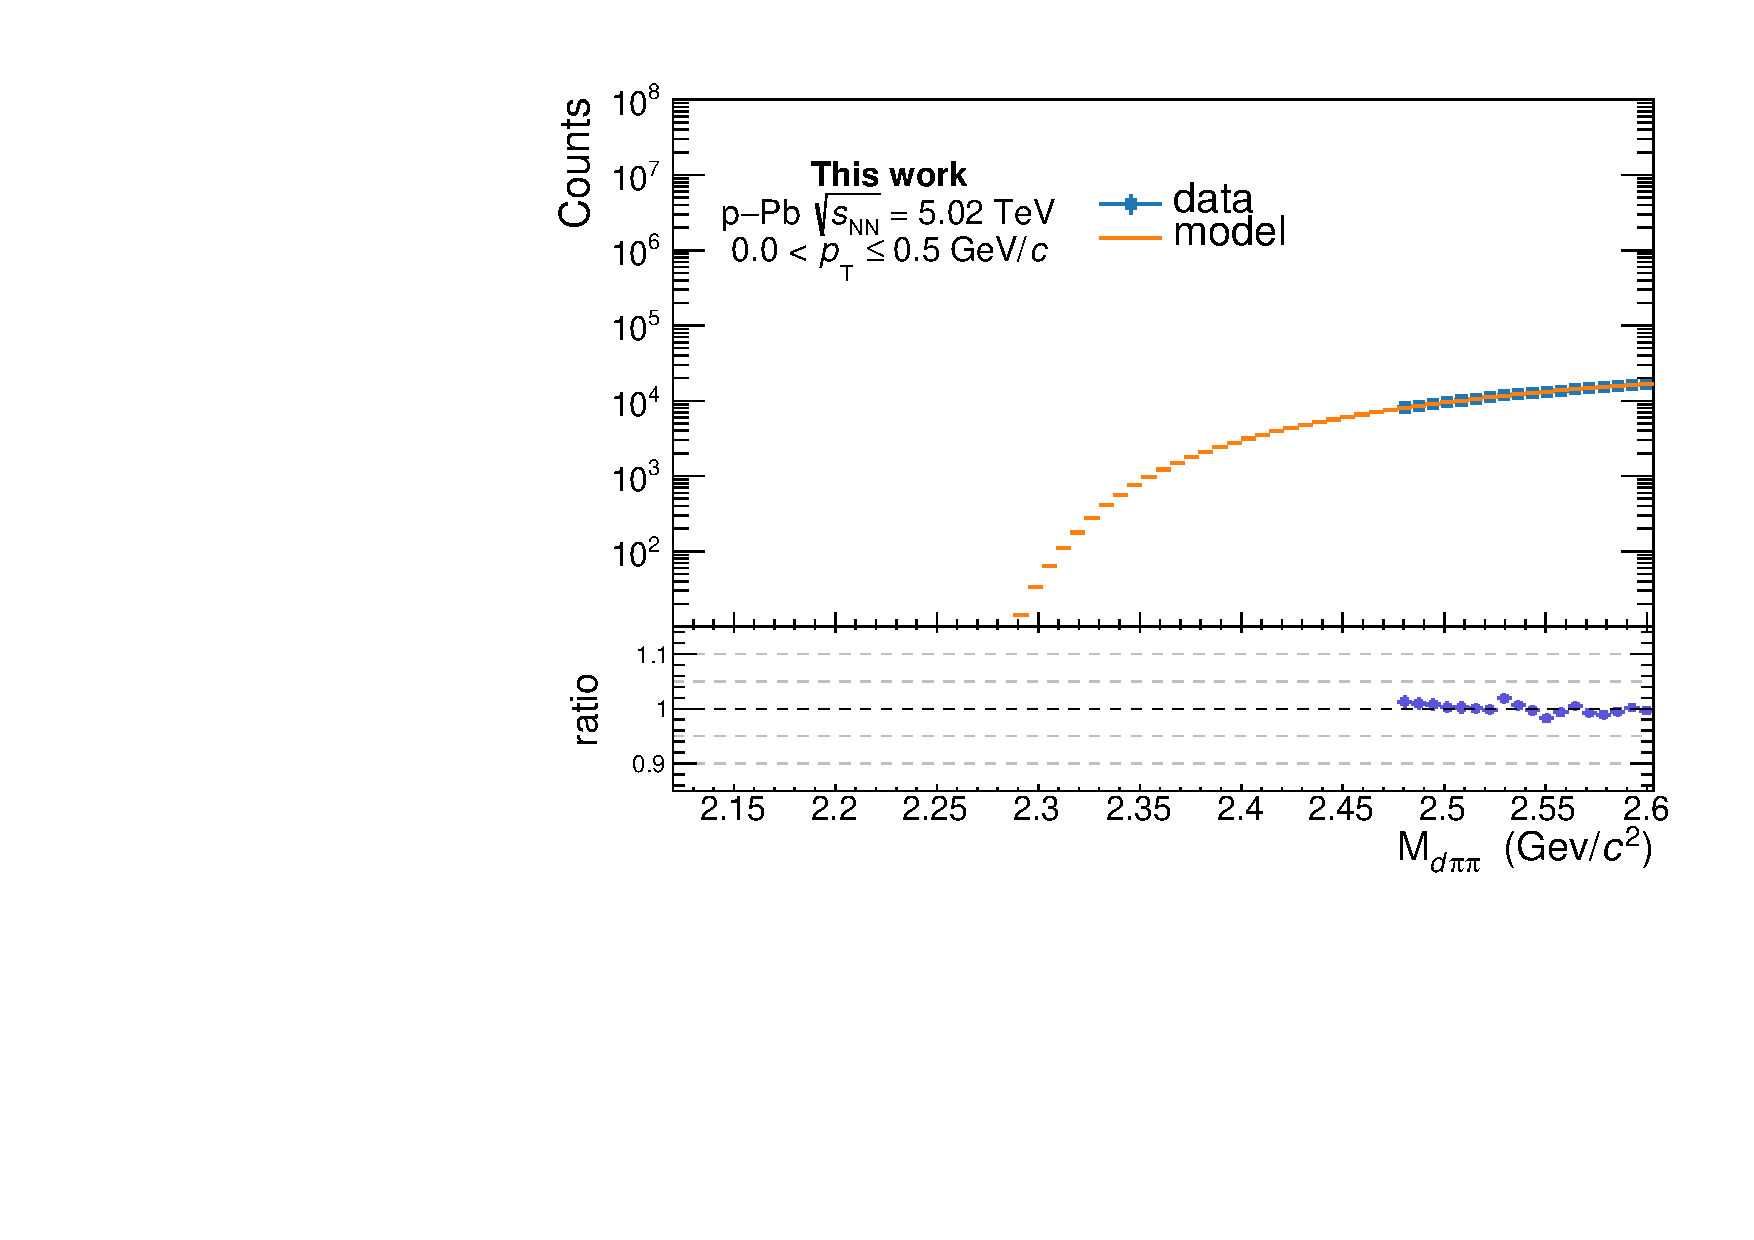
\includegraphics[width=\linewidth]{gfx/appendix/can_blind0}
  \caption{}
\end{subfigure}%
\begin{subfigure}{.5\textwidth}
  \centering
  \captionsetup{justification=centering}
  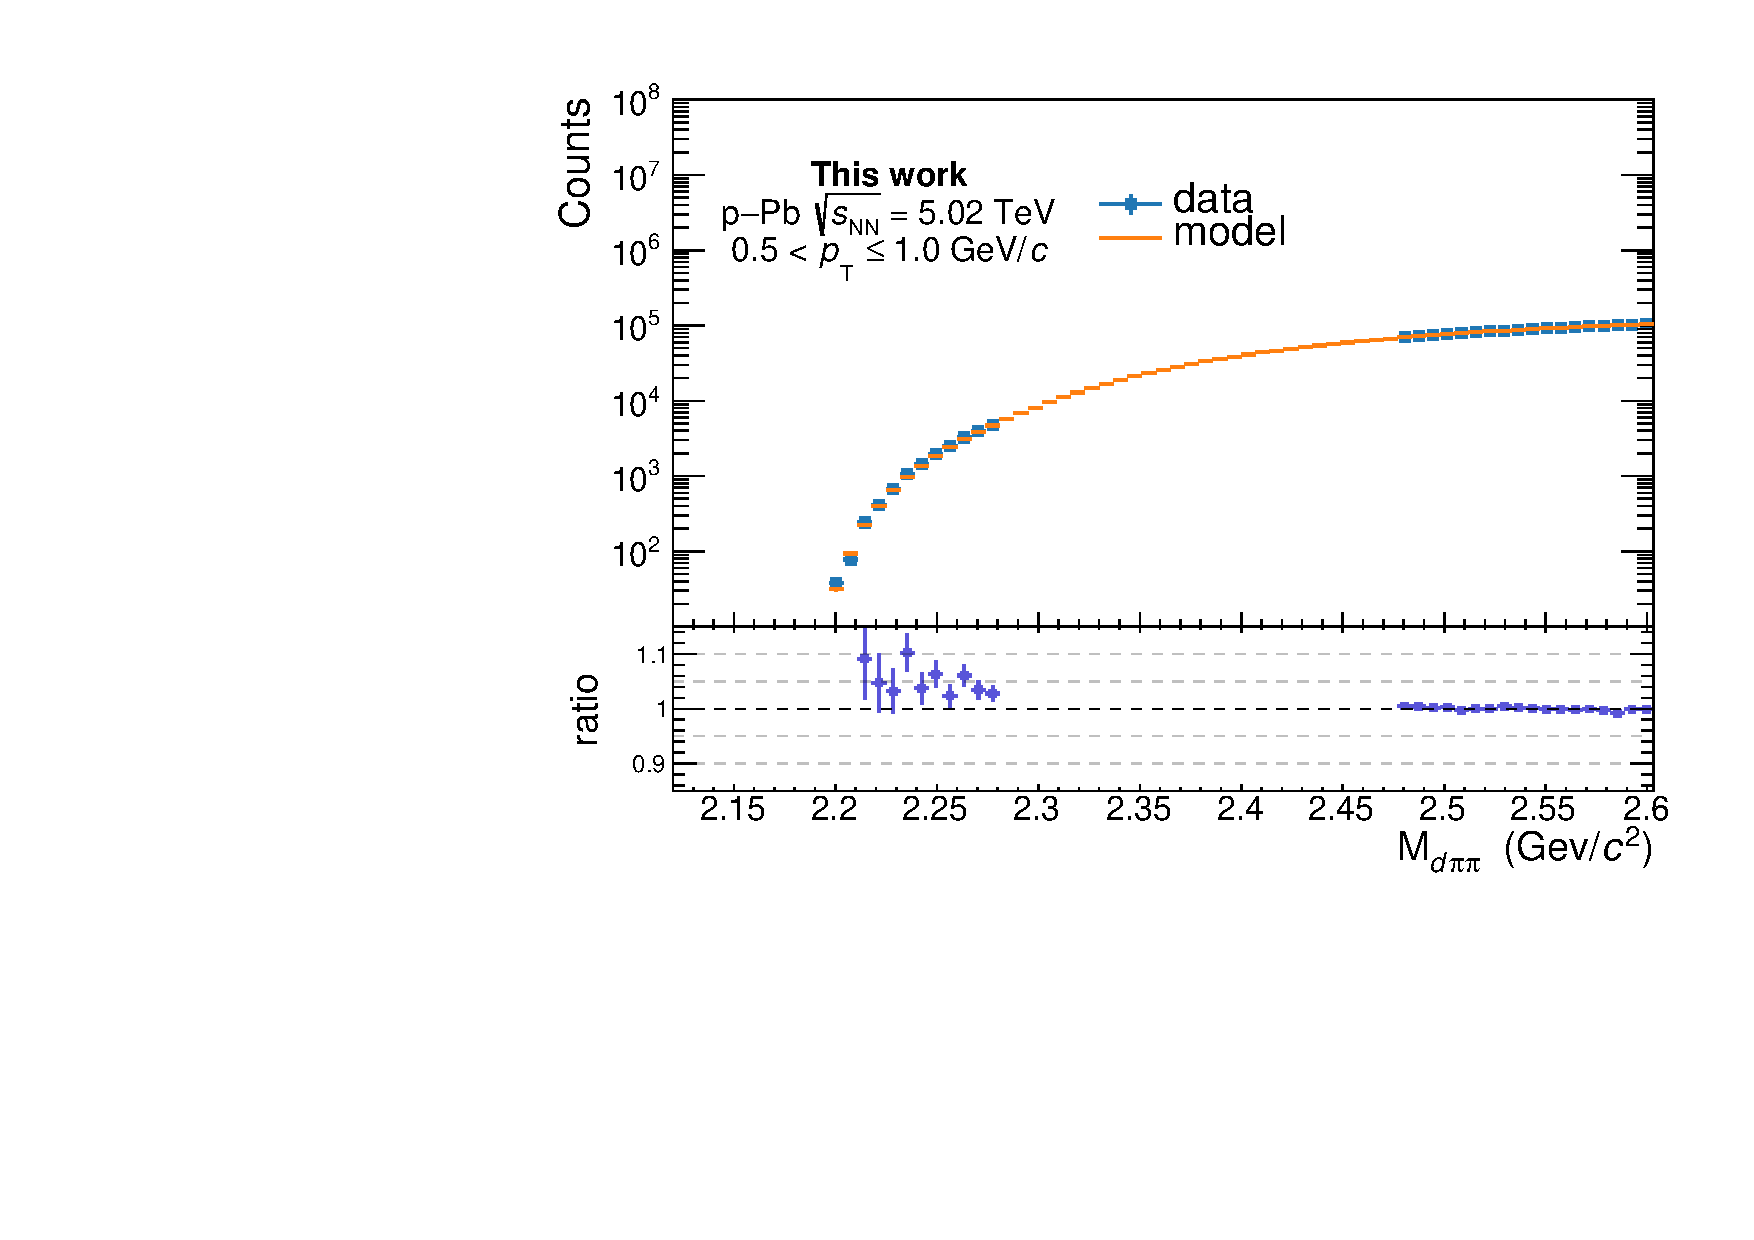
\includegraphics[width=\linewidth]{gfx/appendix/can_blind1}
  \caption{}
\end{subfigure}
\caption{Expected transverse momentum spectrum for the \ds decay product derived with the rejection sampling: pions in panel (a) and deuterons in panel (b).}
\label{fig:BW_spec_prod}
\end{figure}

\begin{figure}[htb]
\begin{subfigure}{.5\textwidth}
  \centering
  \captionsetup{justification=centering}
  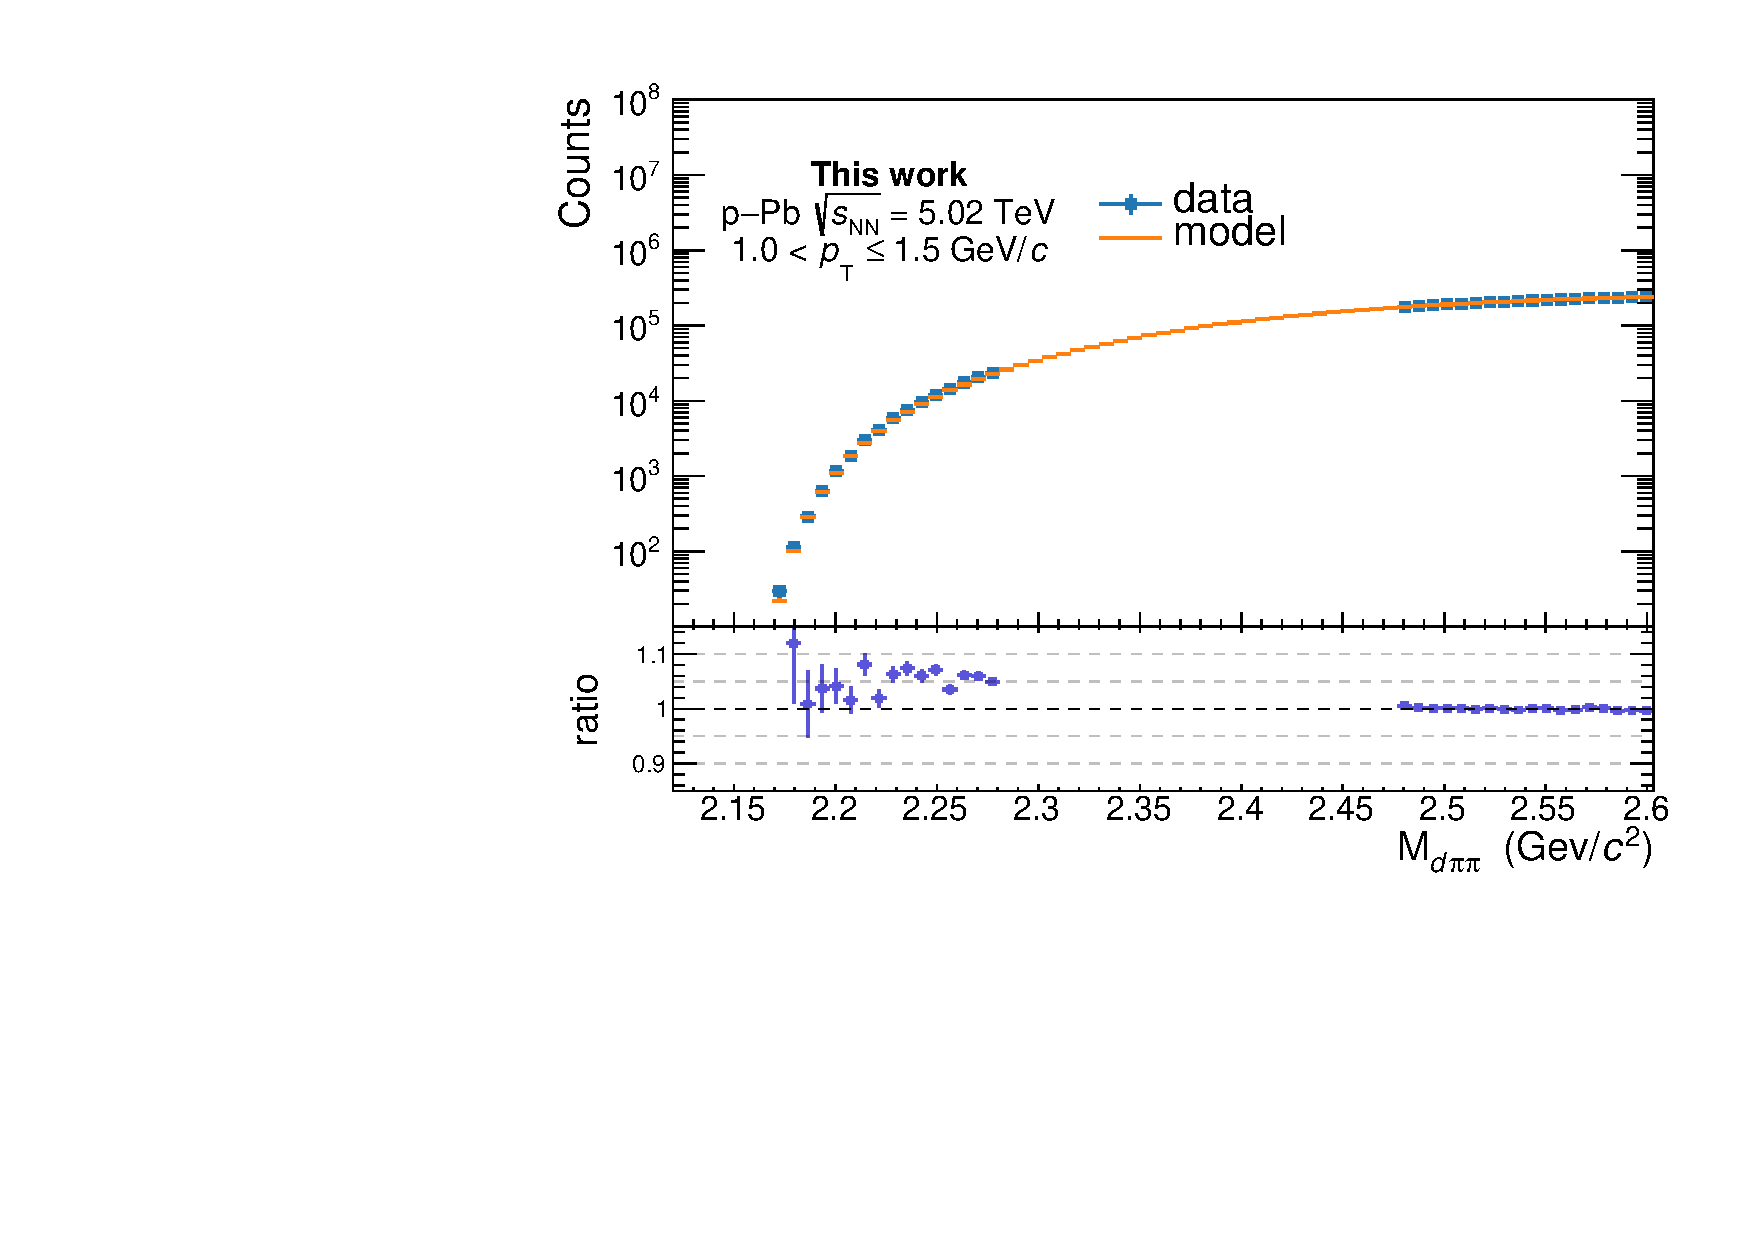
\includegraphics[width=\linewidth]{gfx/appendix/can_blind2}
  \caption{}
\end{subfigure}%
\begin{subfigure}{.5\textwidth}
  \centering
  \captionsetup{justification=centering}
  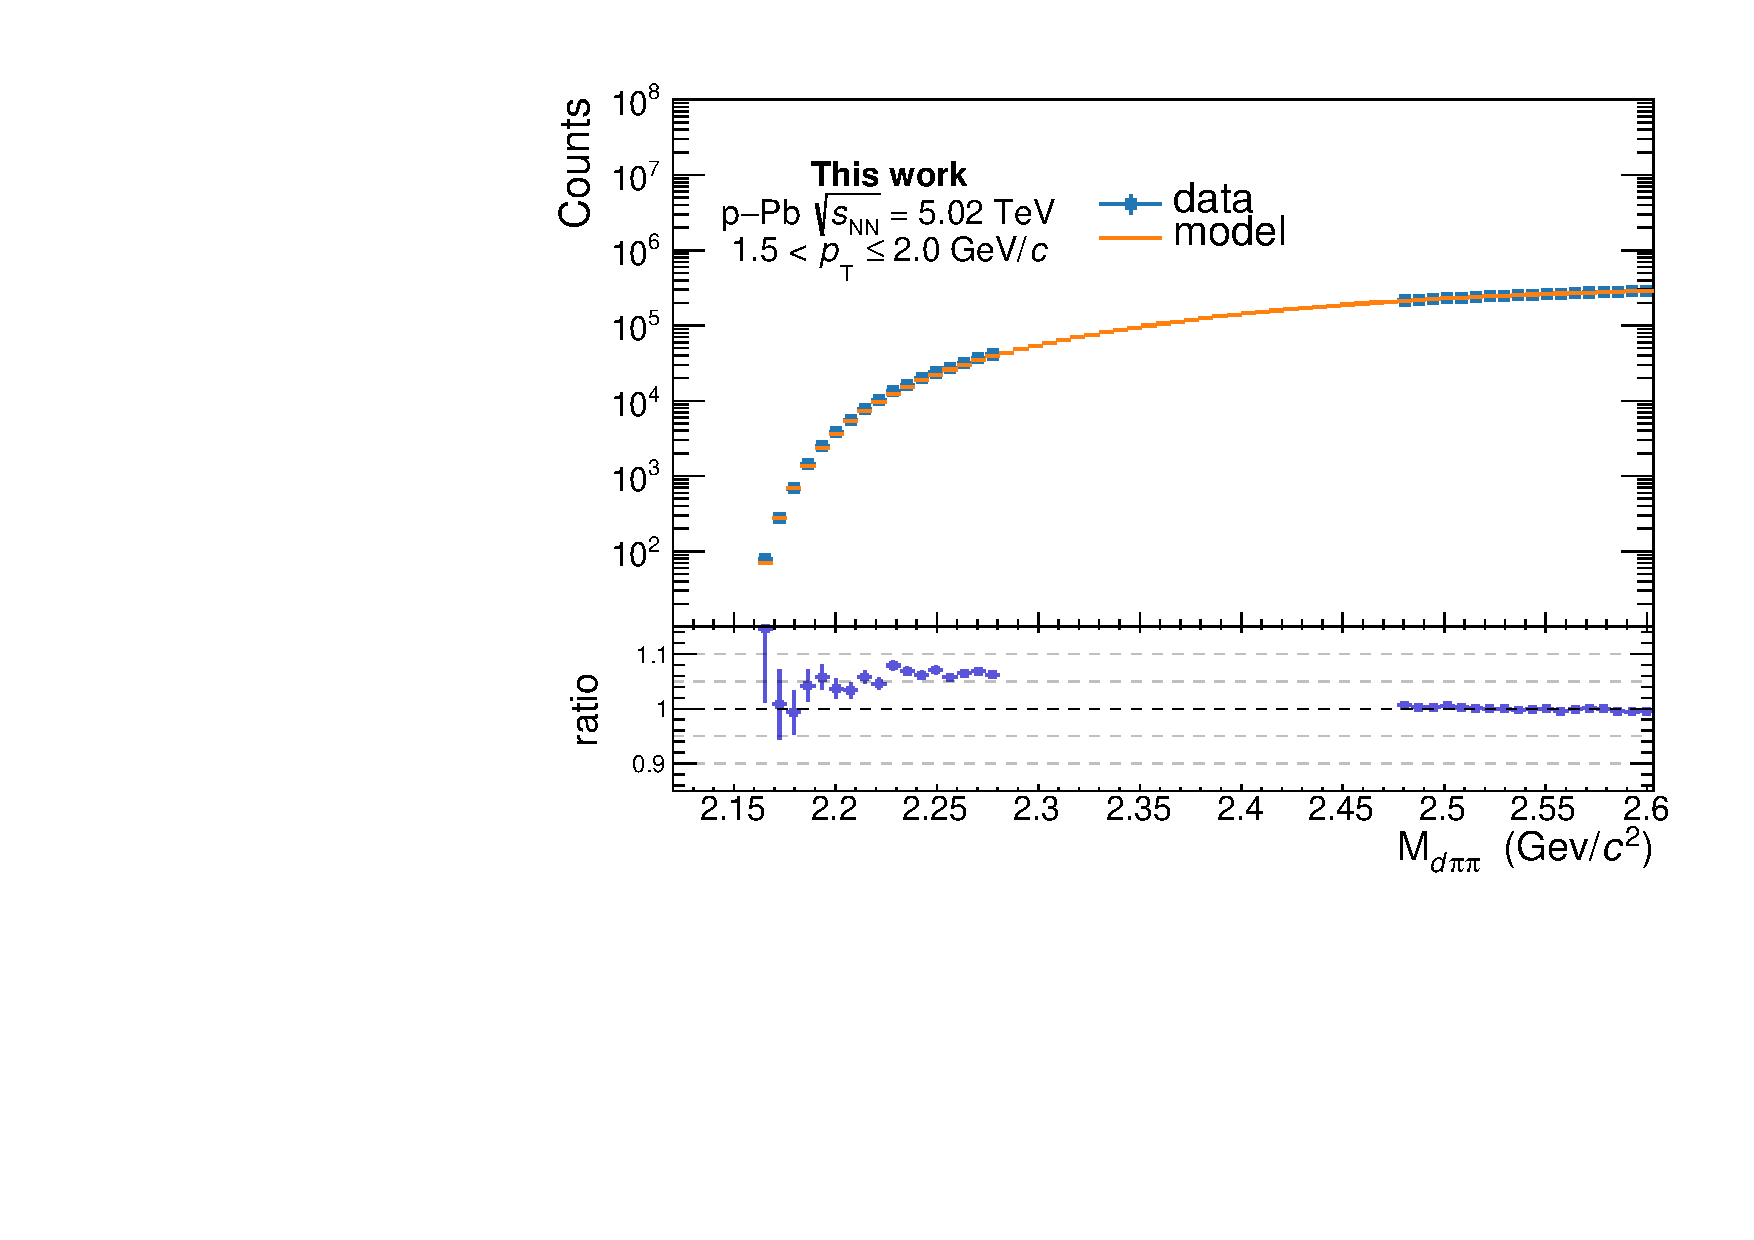
\includegraphics[width=\linewidth]{gfx/appendix/can_blind3}
  \caption{}
\end{subfigure}

\begin{subfigure}{.5\textwidth}
  \centering
  \captionsetup{justification=centering}
  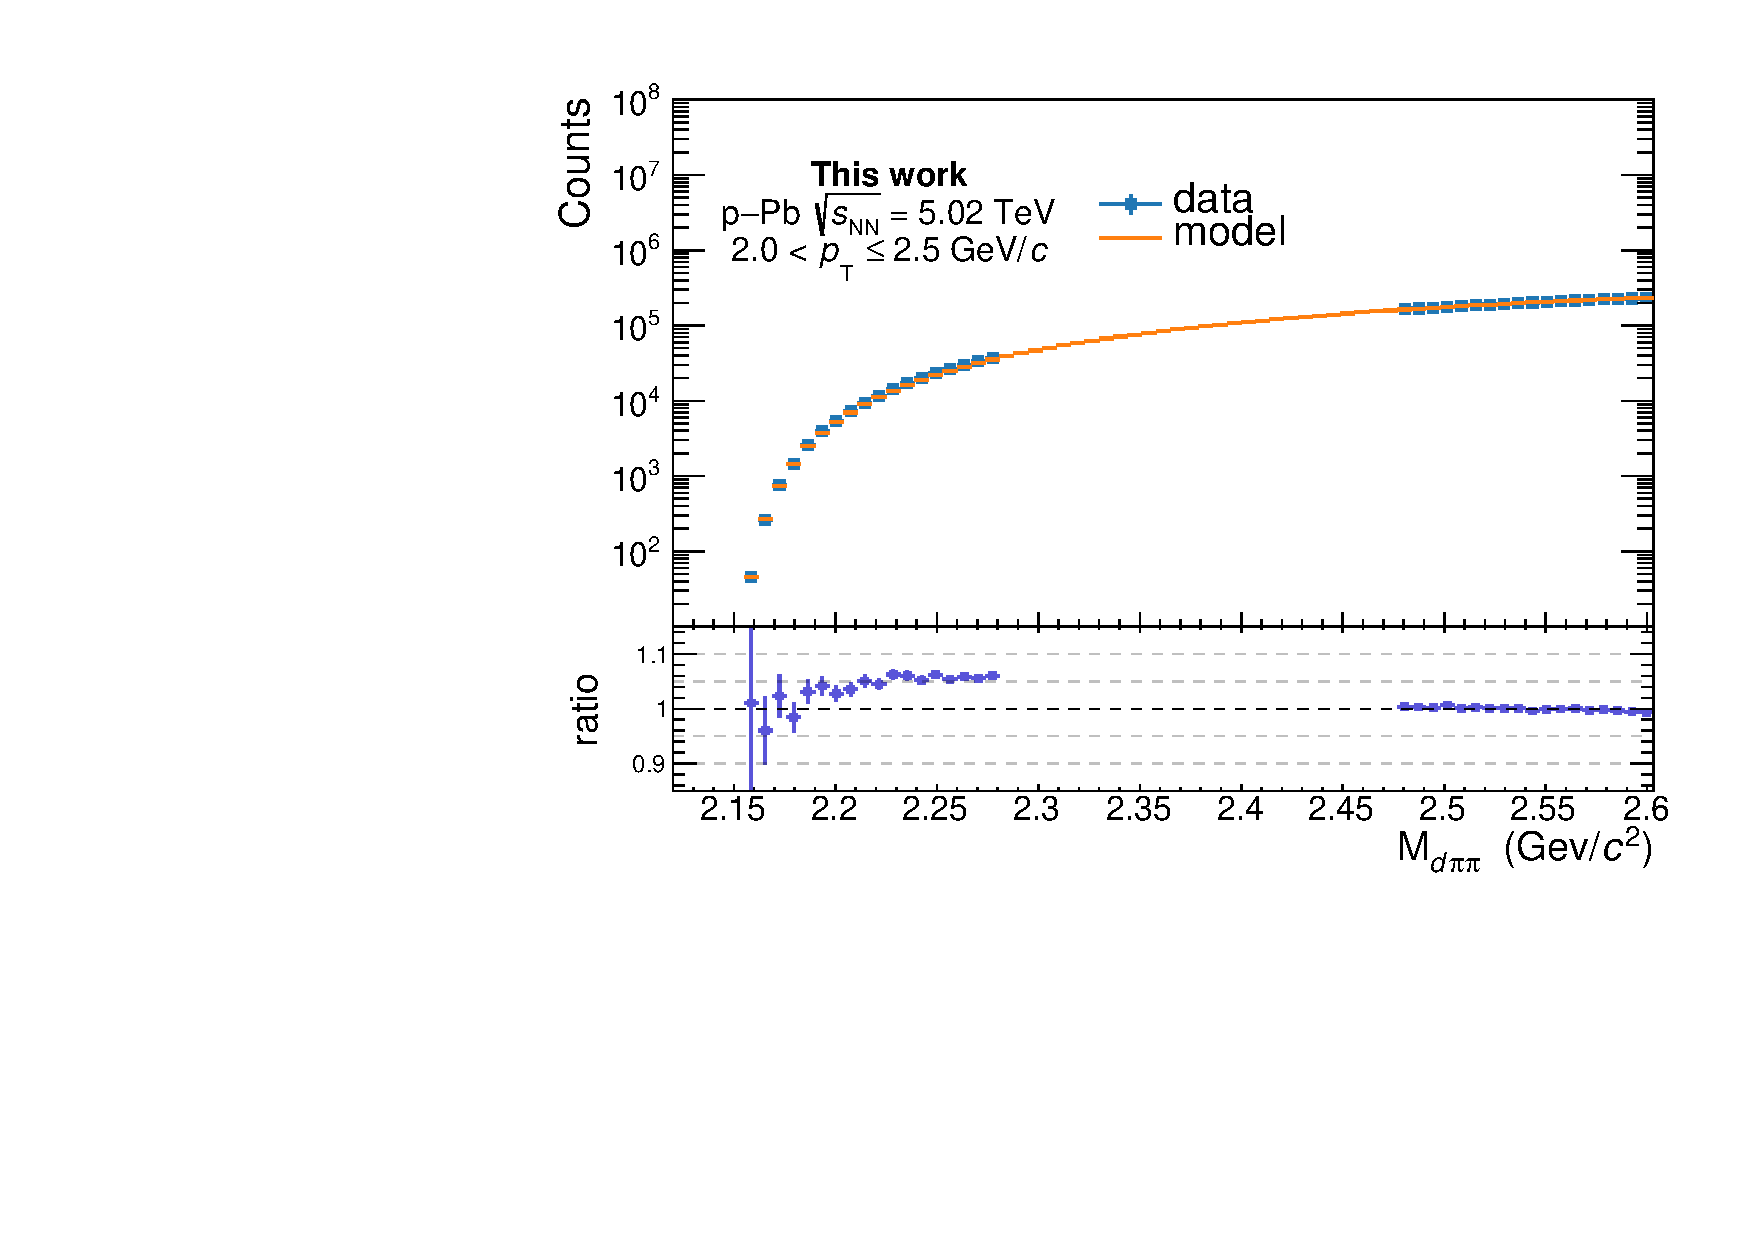
\includegraphics[width=\linewidth]{gfx/appendix/can_blind4}
  \caption{}
\end{subfigure}%
\begin{subfigure}{.5\textwidth}
  \centering
  \captionsetup{justification=centering}
  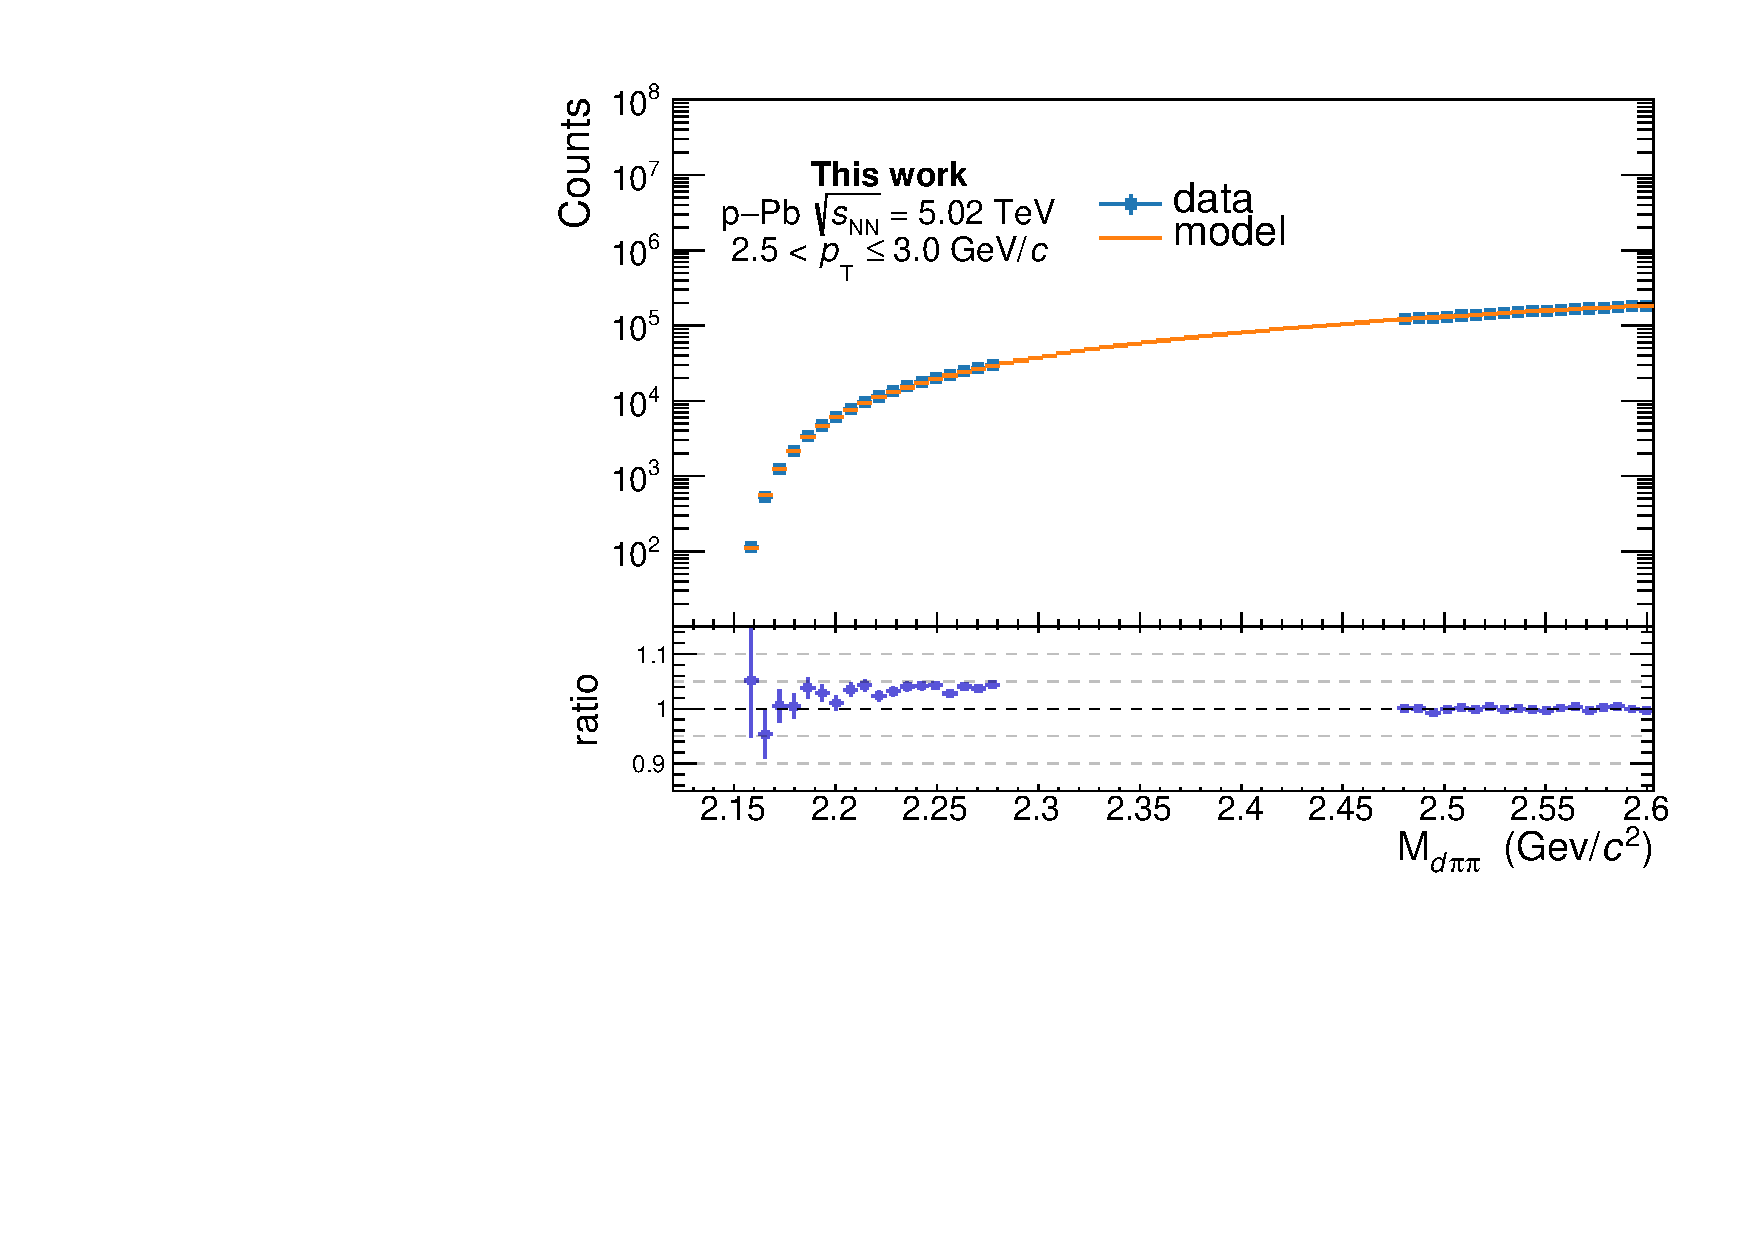
\includegraphics[width=\linewidth]{gfx/appendix/can_blind5}
  \caption{}
\end{subfigure}
\begin{subfigure}{.5\textwidth}
  \centering
  \captionsetup{justification=centering}
  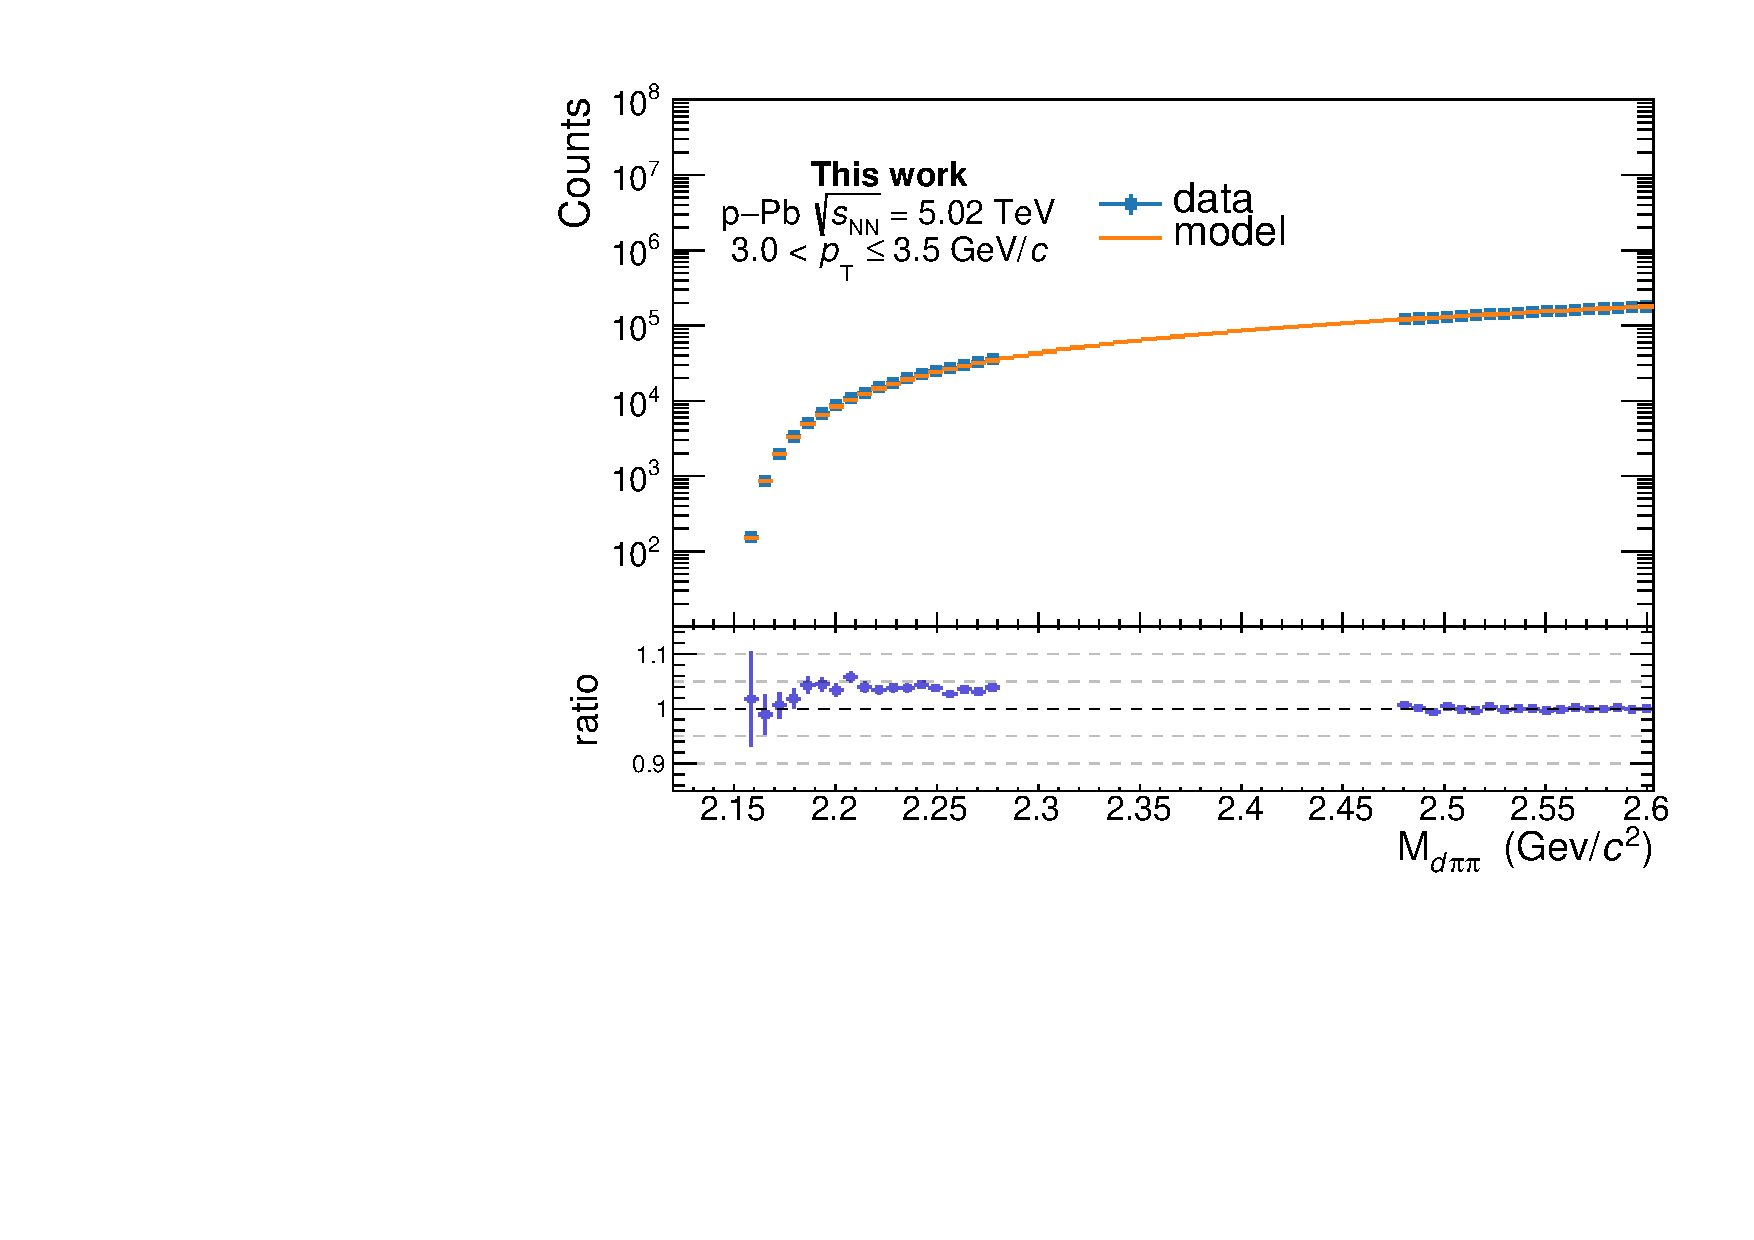
\includegraphics[width=\linewidth]{gfx/appendix/can_blind6}
  \caption{}
\end{subfigure}%
\begin{subfigure}{.5\textwidth}
  \centering
  \captionsetup{justification=centering}
  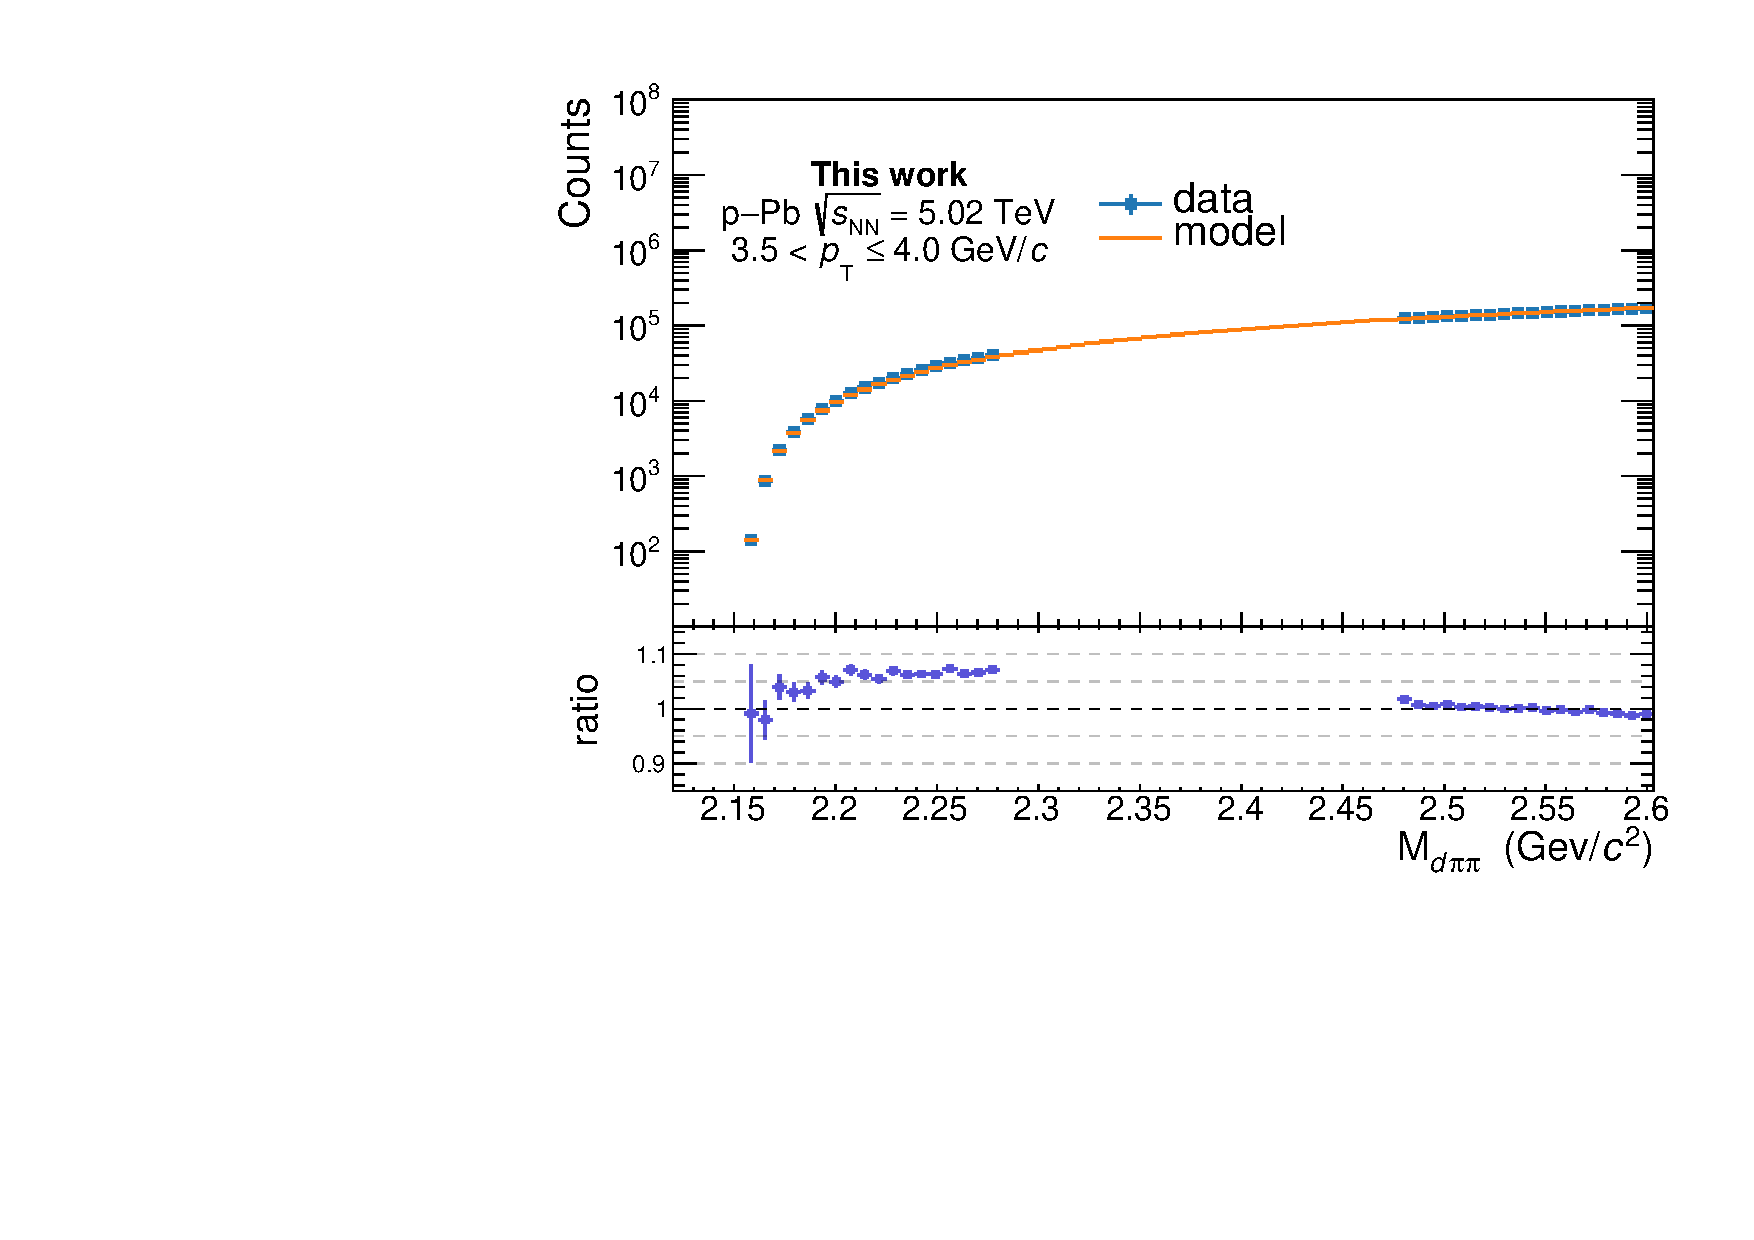
\includegraphics[width=\linewidth]{gfx/appendix/can_blind7}
  \caption{}
\end{subfigure}
\caption{Expected transverse momentum spectrum for the \ds decay product derived with the rejection sampling: pions in panel (a) and deuterons in panel (b).}
\label{fig:BW_spec_prod}
\end{figure}

\begin{figure}[htb]
\begin{subfigure}{.5\textwidth}
  \centering
  \captionsetup{justification=centering}
  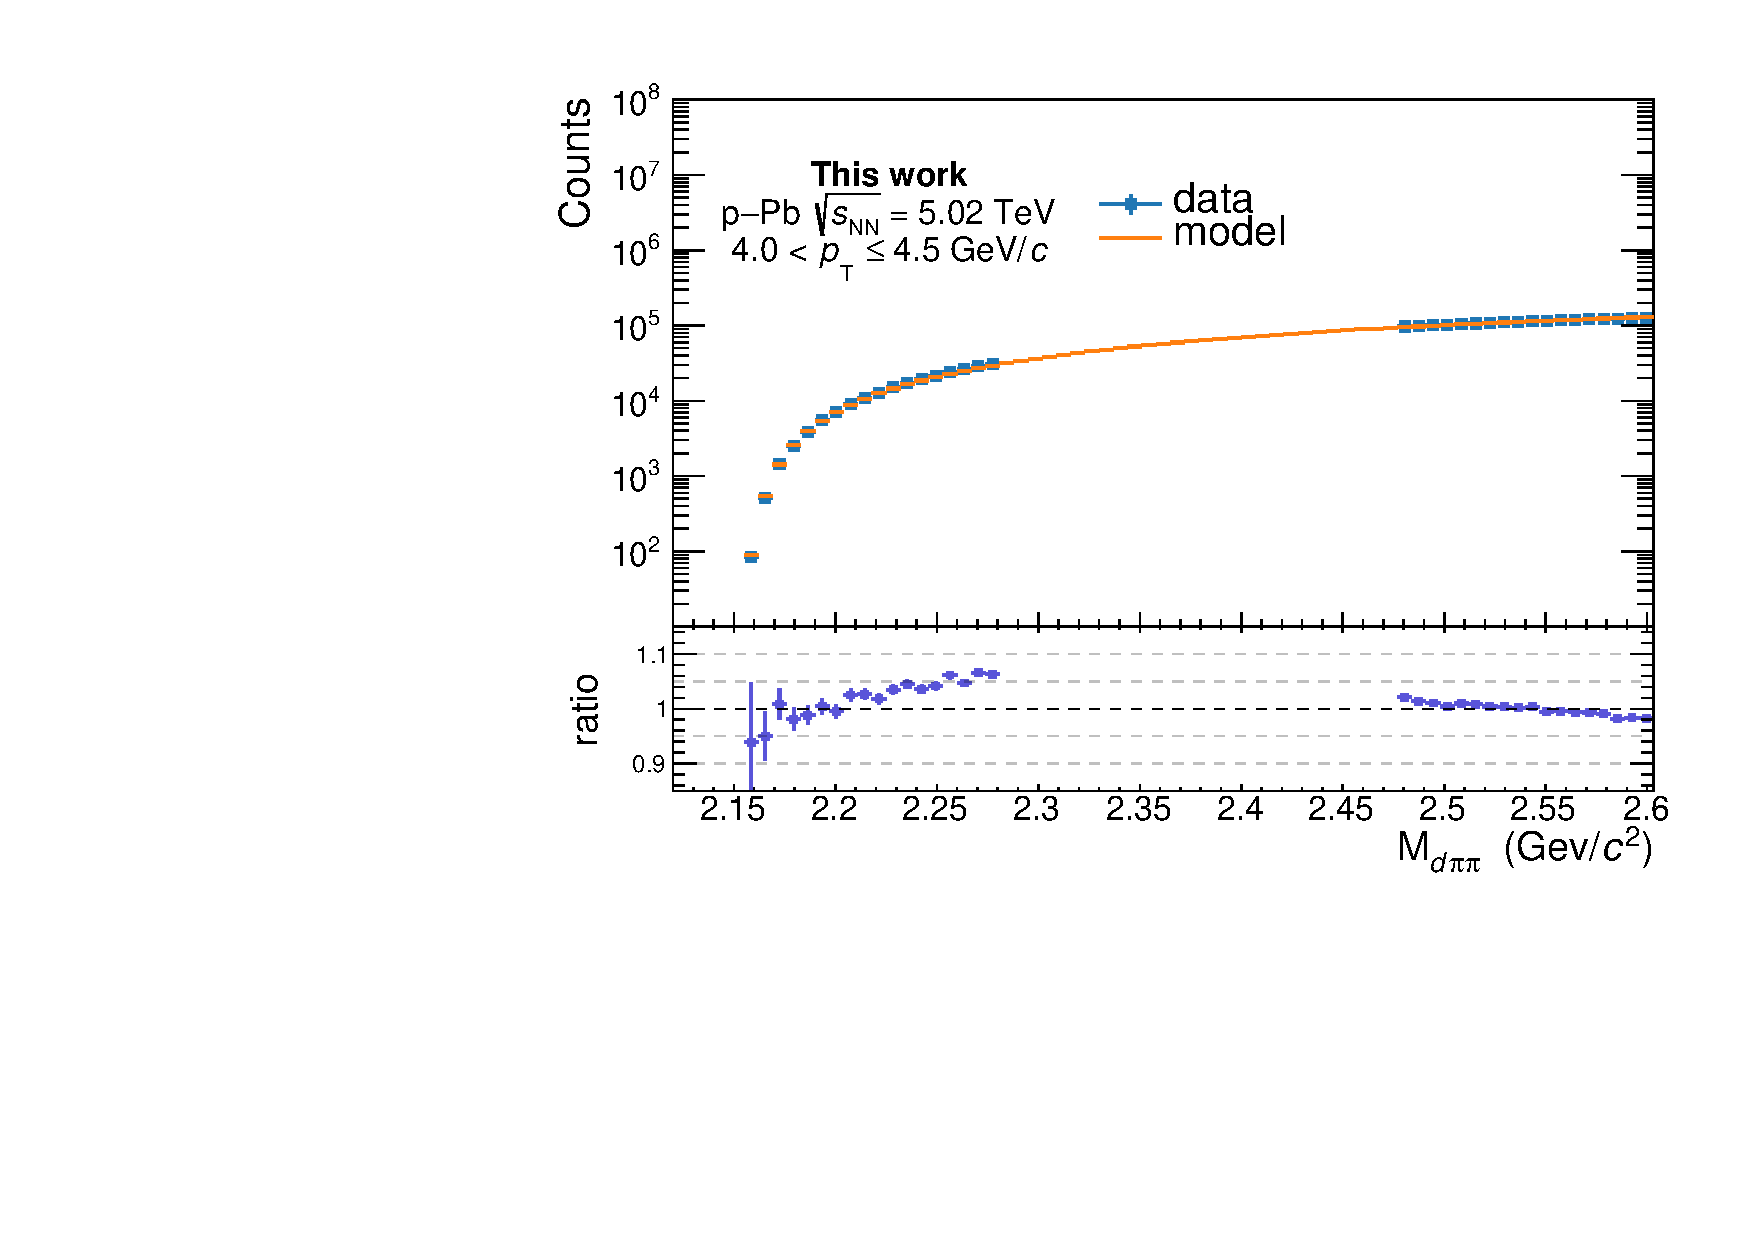
\includegraphics[width=\linewidth]{gfx/appendix/can_blind8}
  \caption{}
\end{subfigure}%
\begin{subfigure}{.5\textwidth}
  \centering
  \captionsetup{justification=centering}
  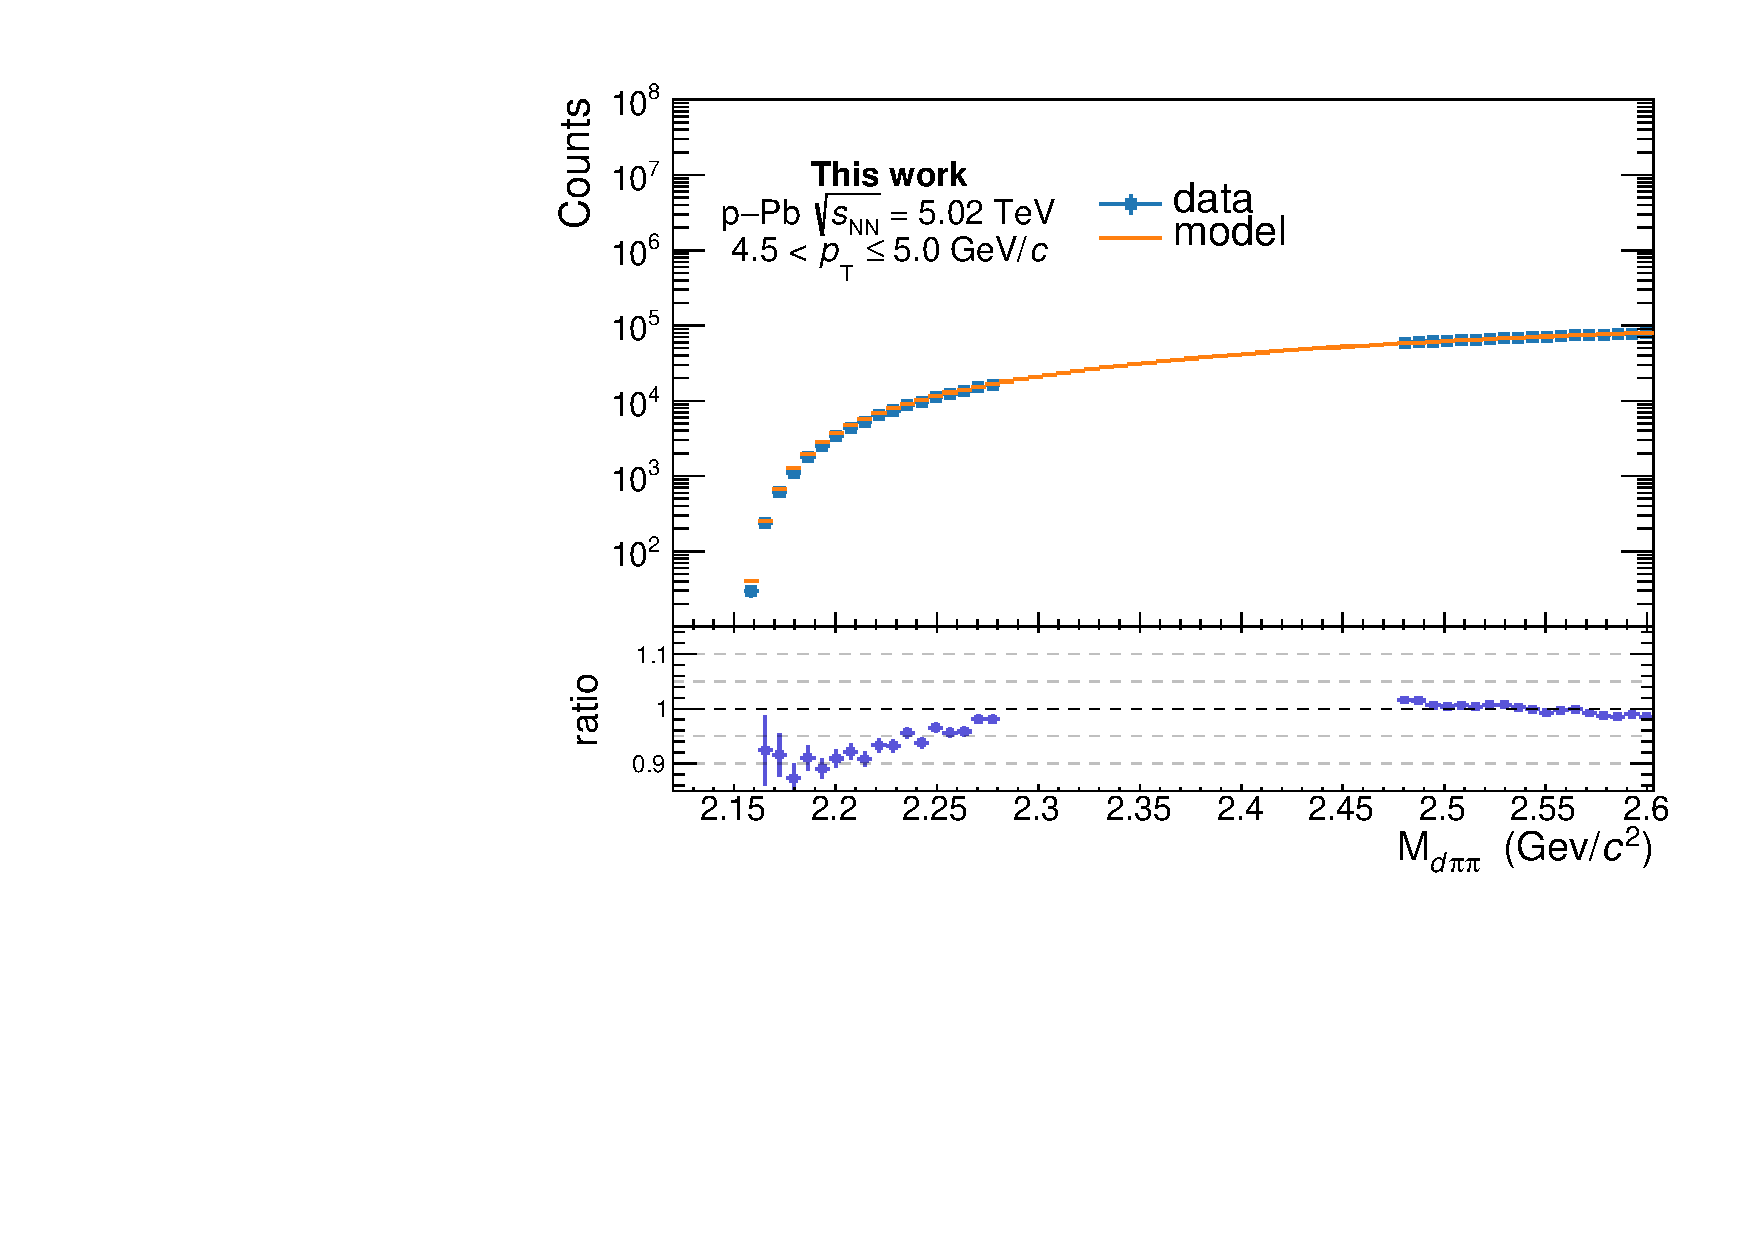
\includegraphics[width=\linewidth]{gfx/appendix/can_blind9}
  \caption{}
\end{subfigure}
\caption{Expected transverse momentum spectrum for the \ds decay product derived with the rejection sampling: pions in panel (a) and deuterons in panel (b).}
\label{fig:BW_spec_prod}
\end{figure}

%
\subsection*{PEM model additional plot} \label{app:pemimp}


%
%
\section*{Background subtraction} \label{app:bsub}


\end{appendices}